\section{Installing FALCON}

\section{Running FALCON}

There are several ways to run FALCON. The script that implements
Algorithm~\ref{alg:FALCON} is \textit{falcon.m}; this script takes
many optional values, and the function signature is highly likely
to change in the near future. For basic use, we suggest using
the wrapper script \textit{runFalcon.m}, which assumes several
parameter values. This wrapper could be easily changed to use
different parameter defaults, or to call \textit{falconMulti.m},
itself a wrapper with a similar function signature for
\textit{falcon.m} that calculates the mean and standard deviation of
fluxes across multiple calls to \textit{falcon.m}.

\section{Assumptions for enzyme complex formation}
\label{sec:complexation}

In order to quantify enzyme complex formation (sometimes called enzyme
complexation), the notion of an enzyme complex should be formalized.
A protein complex typically refers to two or more physically
associated polypeptide chains, which is sometimes called a quaternary
structure. Since we are not exclusively dealing with multiprotein
complexes, we refer to an enzyme complex as being one or more
polypeptide chains that act together to carry out metabolic
catalysis.

\emph{Assumption~\ref{asm:expcorr}.}  The first assumption that we
need in order to guarantee an accurate estimate of (relative) enzyme
complex copy number are accurate measurements of their component
subunits. Unfortunately, this is currently not possible, and we almost
always must make do with mRNA measurements, which may even have some
degree of inaccuracy in measuring the mRNA copy number. What has been
seen is that Spearman's $\rho = 0.6$ for correlation between RNA-Seq
and protein inensity in datasets from HeLa cells
\citep{Nagaraj2011}. This implies that much can likely still be
gleamed from analyzing RNA-Seq data, but, an appropriate degree of
caution must be used in interpreting results based on RNA-Seq data. By
incorporating more information, such as metabolic constaints, we hope
to obviate some of the error in estimating protein intensity from
RNA-Seq data.  

\emph{Assumption~\ref{asm:isozyme}.} We also include the notion of
isozymes--different proteins that catalyze the same reaction--in our
notion of enzyme complex. Isozymes may arise by having one or more
differing protein isoforms, and even though these isoforms may not be
present in the same complex at the same moment, we consider them to be
part of the enzyme complex since one could be substituted for the
other.

As an example for assumptions described so far, take the $F_1$
subcomplex of ATP Synthase (Figure ~\ref{fig:2F43}), which is composed
of seven protein subunits (distinguised by color, left). On the
right-hand side we see different isoforms depicted as different
colors.  Error in expression data aside, instead of considering the
copy numbers with multiplicity and dividing their expression values by
their multiplicity, it may be easier to simply note that the axle
peptide (shown in red in the center of the complex) only has one copy
in the complex, so its expression should be an overall good estimation
of the $F_1$ subcomplex copy number. This reasoning will be useful
later in considering why GPRs may be largely adequate for estimating
the abundance of most enzyme complexes.

\begin{figure*}%[H]
\label{fig:2F43}
\centering
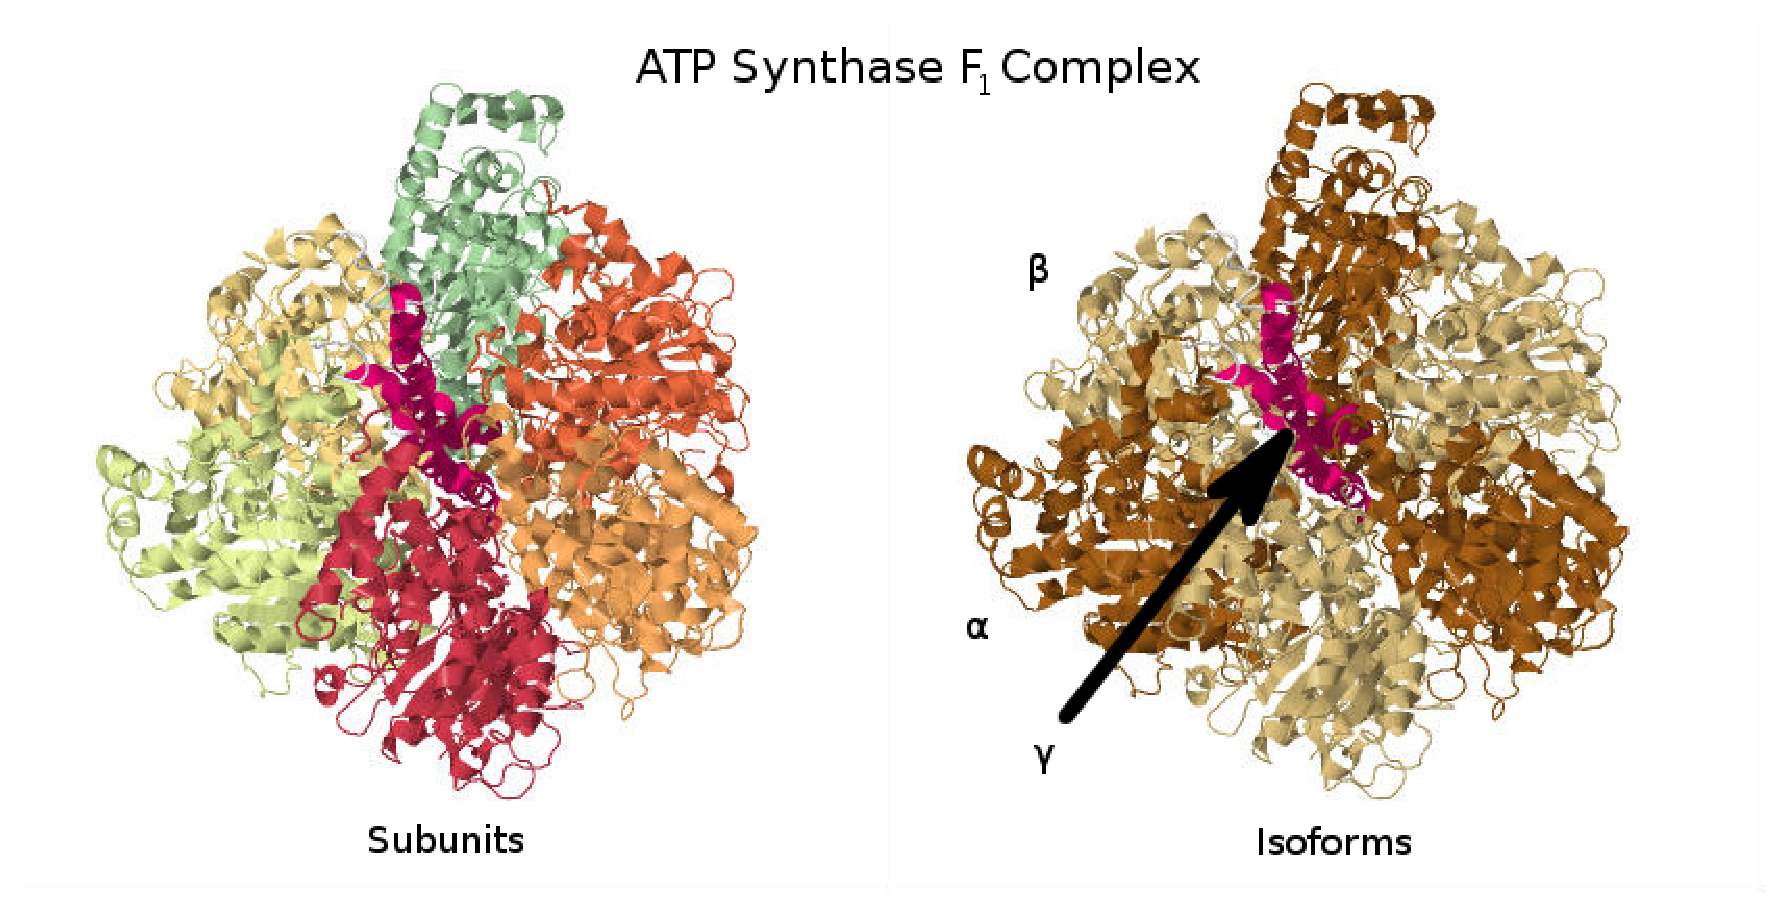
\includegraphics[clip=true,trim=0cm 0cm 0cm 0cm, width=12cm]{2F43}
\caption{Illustration of the $F_1$ part of the ATP Synthase complex
  (PDB ID 1E79; \citealt{Gibbons2000,Bernstein1978,Gezelter}).
  This illustration demonstrates both how an enzyme complex may be
  constituted by multiple subunits (left), and how some of those
  subunits may be products of the same gene and have differing
  stoichiometries within the complex (right).}
\end{figure*}

\emph{Assumption~\ref{asm:hierarchy}.}

The modeling of enzyme complex copy number can be tackled by using
nested sets of subcomplexes; each enzyme complex consists of multiple
subcomplexes, unlesss it is only a single protein or family of protein
isozymes.  These subcomplexes are required for the enzyme complex to
function (AND relationships), and can be thought of as the division of
the complex in to distinct units that each have some necessary
function for the complex, with the exception that we do not keep track
of the multiplicity of subcomplexes within a complex since this
information is, in the current state of affairs, not always known.
However, there may be alternative versions of each functional set
(given by OR relationships). Eventually, this nested embedding
terminates with a single protein or set of peptide isoforms
(e.g.\ isozymes).  In the case of ATP Synthase, one of its functional
sets is represented by the $F_1$ subcomplex. The $F_1$ subcomplex
itself can be viewed as having two immediate subcomplexes: the single
$\gamma$ (axle) subunit and three identical subcomplexes each made of
an $\alpha$ and $\beta$ subunit. Each $\alpha\beta$ pair works
together to bind ADP and catalyze the reaction \citep{Oster2003}. The
$\alpha\beta$ subcomplex itself then has two subcomplexes composed of
just an $\alpha$ subunit on the one hand and the $\beta$ subunit on
the other.  It is obvious that one of these base-level functional
subcomplexes (in this example, either $\gamma$ or $\alpha\beta$) will
be in most limited supply, and that it will best represent the overall
enzyme complex copy number (discounting the issues of multiplicity for
$\alpha\beta$, discussed above).

%
% Consider adding this as a Theorem/Proof:
%

The hierarhical structure just described, when written out in Boolean,
will give a rule in CNF (conjunctive normal form). This is because all
relations are ANDs (conjunctions), except possibly at the inner-most
subcomplexes that have alternative isoforms, which are expressed as
ORs (disjunctions). Since GPR rules alone only specify the
requirements for enzyme complex formation, we will see that not all
forms of boolean rules are equally useful in evaluating the enzyme
complex copy number, but we have established the assumptions in
Table~\ref{ECAssume} and an alternative and logically equivalent rule
\citep{Russell2009} under which we can estimate enzyme complex copy
number.


\def \ECAssumeCap {Assumptions in GPR-based Enzyme Complex Formation}
\label{ECAssume}
\ifthenelse{\boolean{thesisStyle}}{
  \begin{tabular}{| p{\textwidth} |}
  \hline
  \textbf{Table ~\ref{ECAssume}. \ECAssumeCap} \\
  \hline
  % I put this in to a separate file because formatting the table in different ways
% is difficult; it may even be better to have multiple versions of this table
% for different documents, but hopefully we can avoid such code duplication.

%Internal part of the table:

\begin{enumerate}
% This is really not related to GPR rules: 
%\ifthenelse{\boolean{thesisStyle}}{\item} {} \label{asm:mm}
%Fluxes in general strive to operate near the $V_{max}$ of the
%reaction, which is proportional to enzyme complex abundance.
\item \label{asm:expcorr}
Expression values are highly correlated with the copy numbers of their
corresponding peptide isoforms.
\item \label{asm:isozyme} 
Protein isoforms contributing to isozymes are considered part of the
same enzyme complex.
\item \label{asm:hierarchy}
Any enzyme complex can be described as a hierarchical subset of
(possibly redundant) subcomplexes; redundant subcomplexes, as
elaborated in (\ref{asm:nostoich}), are not currently modeled.
\item \label{asm:nostoich} 
Assume one copy of peptide per complex; exact isoform stoichiometry
is not considered.
\item \label{asm:sharing} 
With the exception of complexes having identical rules (i.e. the same
complex listed for different reactions), each copy of a peptide
is available for all complexes in the model.
\item \label{asm:active_site}
There is only one active site per enzyme complex.
\item \label{asm:enzyme_sensitivity} 
We assume that different pathways have similar flux sensitivities
with respect to their enzyme abundances.
\item \label{asm:holo} 
If a particular subcomplex can be catalyzed by A and it can also be
catalyzed by A and B (e.g. B acts as a regulatory unit, as in
holoenzymes), this just simplifies to A once expression values are
substituted in. Similarly, allosteric regulation is not
modeled. Relatedly, there are no NOT operations in GPR rules (just ANDs
and ORs).
\item \label{asm:chap} 
Enzyme complexes form without the assistance of protein chaperones and
formation is not coupled to other reactions.
\item \label{asm:posttrans}
Post-translational modifications do not affect complex formation.
\item \label{asm:rate} 
Rate of formation and degradation of complexes doesn't play a role,
since we assume steady-state. 
\end{enumerate}

  \\ \hline
  \end{tabular}

} {
  % For Bioinformatics:
  \begin{table*}[!t]
  \processtable{\ECAssumeCap \label{ECAssume}}{
  \begin{tabular}{| p{\textwidth} |}
  \hline
  % I put this in to a separate file because formatting the table in different ways
% is difficult; it may even be better to have multiple versions of this table
% for different documents, but hopefully we can avoid such code duplication.

%Internal part of the table:

\begin{enumerate}
% This is really not related to GPR rules: 
%\ifthenelse{\boolean{thesisStyle}}{\item} {} \label{asm:mm}
%Fluxes in general strive to operate near the $V_{max}$ of the
%reaction, which is proportional to enzyme complex abundance.
\item \label{asm:expcorr}
Expression values are highly correlated with the copy numbers of their
corresponding peptide isoforms.
\item \label{asm:isozyme} 
Protein isoforms contributing to isozymes are considered part of the
same enzyme complex.
\item \label{asm:hierarchy}
Any enzyme complex can be described as a hierarchical subset of
(possibly redundant) subcomplexes; redundant subcomplexes, as
elaborated in (\ref{asm:nostoich}), are not currently modeled.
\item \label{asm:nostoich} 
Assume one copy of peptide per complex; exact isoform stoichiometry
is not considered.
\item \label{asm:sharing} 
With the exception of complexes having identical rules (i.e. the same
complex listed for different reactions), each copy of a peptide
is available for all complexes in the model.
\item \label{asm:active_site}
There is only one active site per enzyme complex.
\item \label{asm:enzyme_sensitivity} 
We assume that different pathways have similar flux sensitivities
with respect to their enzyme abundances.
\item \label{asm:holo} 
If a particular subcomplex can be catalyzed by A and it can also be
catalyzed by A and B (e.g. B acts as a regulatory unit, as in
holoenzymes), this just simplifies to A once expression values are
substituted in. Similarly, allosteric regulation is not
modeled. Relatedly, there are no NOT operations in GPR rules (just ANDs
and ORs).
\item \label{asm:chap} 
Enzyme complexes form without the assistance of protein chaperones and
formation is not coupled to other reactions.
\item \label{asm:posttrans}
Post-translational modifications do not affect complex formation.
\item \label{asm:rate} 
Rate of formation and degradation of complexes doesn't play a role,
since we assume steady-state. 
\end{enumerate}

  \\ \hline
  \end{tabular}
  }
  {} % caption
  \end{table*}
}

There is no guarantee that a GPR rule has been written down with this
hierarchical structure in mind, though it is likely the case much of
the time as it is a natural way to model complexes.  However, any GPR
rule can be interpreted in the context of this hierarchical view due
to the existence of a logically equivlaent CNF rule for any non-CNF
rule, and it is obvious that logical equivalence is all that is
required to check for enzyme complex formation when exact isoform
stoichiometry is unknown.  As an example, we consider another common
formulation for GPRs, and a way to think about enzyme
structure---disjunctive normal form (DNF).  A DNF rule is a
disjunctive list of conjunctions of peptide isoforms, where each
conjunction is some variation of the enzyme complex due to
substituting in different isoforms for some of the required
subunits. A rule with a more complicated structure and compatible
isoforms across subcomplexes may be written more succinctinly in CNF,
whereas a rule with only very few alternatives derived from isoform
variants may be reprsented clearly with DNF.  In rare cases, it is
possible that a GPR rule is written in neither DNF or CNF, perhaps
because neither of these two alternatives above are stricly the case,
and some other rule is more succinct.

\emph{Assumptions~\ref{asm:nostoich},~\ref{asm:sharing}~and~\ref{asm:active_site}.}
One active site per enzyme complex implies a single complex can only
catalyze one reaction at a time. Multimeric complexes with one active
site per identical subunit would be considered as one enzyme complex
per subunit in this model.  Note that it is possible for an enzyme
complex to catalyze different reactions. In fact, some transporter
complexes can transfer many different metabolites \hl{across a lipid
  bilayer---up to X in the case of Y}. Another example is the ligation or hydrolysis of
nucleotide, fatty acid, or peptide chains, where chains of different
length may all be substrates or products of the same enzyme
complex. While we do not explicitly consider these in
Algorithm~\ref{alg:ReductionToCNF}, these redundancies are taken into
account subsequently in Algorithm~\ref{alg:FALCON}.

What is currently not considered in our process is that some peptide
isoforms may find use in completely different complexes, and in some
cases, individual peptides may have multiple active sites; in the
first case, we assume an unrealistic case of superposition where the
isoform can simultaneously function in more than one complex. The
primary reason we have not tackled this problem is because exact
subunit stoichiometry of most enzyme complexes is not accurately
known, but an increasing abundance of data on BRENDA
\citep{Schomburg2013} gives some hope to this problem. A recent
\textit{E. coli} metabolic model incorporating the metabolism of all
known gene products \citep{O'Brien2013} also includes putative
enzyme complex stoichiometry in GPRs. For the second point, there
are a few enzymes where a single polpeptide may have multiple active
sites (e.g.\ fatty acid synthase), and this is not currently taken into
account in our model.

\emph{Assumption~\ref{asm:holo}.}
We do not make any special assumptions requiring symmetry of an
isoform within a complex. For instance, the example in
assumption~\ref{asm:holo} shows how you might have one subcomponent
composed of a single isoform, and another subcomponent composed of
that gene in addition to another isoform. In this case, it is simply
reduced to being the first gene only that is required, since clearly
the second is strictly optional. That isn't to say that the second
gene may not have some effect, such as (potentially) aiding in
structural ability or altering the catalytic rate, but it should have
no bearing on the formation of a functional catalytic
complex. Holoenzymes---enzymes with metabolic cofactors or protein
subunits that have a regulatory function for the complex---would
likely be the only situation where this type of rule might need to be
considered in more detail. But in the absence of detailed kinetic
information, this consideration (much like allosteric
regulation) is not useful.

\emph{Assumptions~\ref{asm:chap}~and~\ref{asm:rate}.}
Due to the quickness, stability, and energetic favorability of enzyme
complex formation, the absence of chaperones or coupled metabolic
reactions required for complex formation may be reasonable
assumptions, but further research is warranted \citep{Karr2012}.
Additionally, as in metabolism, we assume a steady state for complex
formation, so that rate laws regarding complex formation aren't
needed. However, further research may be warranted to investigate the
use of a penalty for complex levels based on mass action and
protein-docking information. Requisite to this would be addressing
assumption~\ref{asm:nostoich}. It would be surprising (but not
impossible) if such a penalty were very larege due to the cost this
would imply for many of the large and important enzyme complexes
present in all organisms \citep{Nelson2008}.

\section{Proof for the minDisjunction algorithm}

Although the logic in the main text may be straightforward, we show
here in more verbosity that Algorithm~\ref{alg:ReductionToCNF} works
as described.

\begin{Theorem}
\label{thm:ReductionToCNF}
Algorithm~\ref{alg:ReductionToCNF} returns the disjunction with
minimum expression value among all disjunctions of a rule in CNF.
\end{Theorem}

\begin{proof}
The third step in the while-loop does not affect the
underlying logic, so we only need to consider the effect of step one
on step two.  Let us first consider when expressions $x_1, ..., x_4$
are all literals in step two to cover the most complex case, and that
$x_i^{(e)}$ denotes the expression measurement for gene $x_i$. Assume
WLOG that $x_1 \lor x_3$ attains the minimum expression among the
disjunctions. Then we have:

\begin{align*}
&x_{1}^{(e)} + x_{3}^{(e)} \leq x_{1}^{(e)} + x_{4}^{(e)} \Rightarrow x_{3}^{(e)} \leq x_{4}^{(e)} \\
&x_{1}^{(e)} + x_{3}^{(e)} \leq x_{2}^{(e)} + x_{3}^{(e)} \Rightarrow x_{1}^{(e)} \leq x_{2}^{(e)} 
\end{align*}

Applying this result in conjunction to step one in the while-loop to
the original expression, $(x_1 \land x_2) \lor (x_3 \land x_4)$, we
immediately arrive at $(x_1) \lor (x_3)$, which gives our originally
assumed minimum. To show that this result doesn't depend on the $x_i$
being literals, merely consider repeating this process recursively for
each $x_i$ that is not a literal to arrive at two different
evaluations for $x_i^{(e)}$ (one where each evaluation is done with
reduction, and one where we evaluate entirely without reduction).
Since the process cannot continue indefinitely, eventually there is a
base case involving only literals, and the above result shows that, at
each step, as we backtrack from the base case, both evaluations will
be identical. The desired result is obtained because
Algorithm~\ref{alg:ReductionToCNF} without step one simply yields CNF,
and it follows that adding step one will yield the disjunction with
minimum expression value of the rule in CNF.
\end{proof}

\section{Code excerpt for minimum disjunction algorithm}
\label{sec:code}

The following code is written in ATS, a type-safe language including
syntax similar to SML while having direct access to C types
\citep{ATStypes03}. \texttt{GREXP} describes a datatype that is used
for storing the parse trees of Boolean rules (without negation).  A
\texttt{GREXP} can then be manipulated by the function \texttt{toCNF}
to be converted to a conjunctive normal form. We make use of the
reduction rule mentioned previously by calling the \texttt{minConj}
function. The \texttt{conjunctivize} function is a helper function to
deal with different structures for \texttt{GRconj} and \texttt{GRdisj}
(one is set based, one is parse-tree based; note this described in the
data(view)type defintion). We note that this is a recursive,
functional implementation of Algorithm~\ref{alg:ReductionToCNF}, which
seems more straightforward than a procedural implementation.

\begin{verbatim}
dataviewtype GREXP = 
  | GRgenes of genes
  | GRconj of genes
  | GRconj of (GREXP,GREXP)
  | GRdisj of genes
  | GRdisj of (GREXP,GREXP)

extern
fun toCNF (bexp: GREXP, emap: &gDMap): GREXP

implement
toCNF (bexp, emap): GREXP = let     
  val LR:GREXP = (case+ bexp of 
    | ~GRconj(ex1,ex2) => GRconj (toCNF(ex1,emap),toCNF(ex2,emap))
    | ~GRdisj(ex1,ex2) => GRdisj (toCNF(ex1,emap),toCNF(ex2,emap))   
    | GR => GR):GREXP
  in (case+ LR of  
    | ~GRconj(ex1,ex2) => minConj(GRconj(ex1,ex2),emap) 
    | ~GRdisj(ex1,ex2) => (case+ (ex1,ex2) of
      // Handle disjunctive leaf cases:         
      | (~GRdisj(lx), ~GRgenes(g)) => GRdisj (lx + g) 
      | (~GRgenes(g), ~GRdisj(rx)) => GRdisj (rx + g)
      | (~GRdisj(lx), ~GRdisj(rx)) => GRdisj (lx + rx)
      | (~GRgenes(g1), ~GRgenes(g2)) => GRdisj (g1 + g2)

      // Distribute OR over ANDs:
      | (~GRconj(x1,x2), ~GRconj(g)) => conj1(x1,x2,g,emap) 
      | (~GRconj(g), ~GRconj(x1,x2)) => conj1(x1,x2,g,emap) 
      | (~GRconj(g1), ~GRconj(g2)) => conj2(g1,g2,emap)
      | (~GRconj(lx1,lx2), ~GRconj(rx1,rx2)) => let
        val lx1c = GREXP_copy(lx1)
        val lx2c = GREXP_copy(lx2) 
        val rx1c = GREXP_copy(rx1)
        val rx2c = GREXP_copy(rx2) 
        in GRconj(GRconj(GRconj(toCNF(GRdisj(lx1,rx1),emap), 
          toCNF(GRdisj (lx2, rx1c ),emap)),
          toCNF(GRdisj (lx1c, rx2),emap)), 
          toCNF(GRdisj (lx2c, rx2c),emap)) 
        end

      // Handle e.g.: (.. OR ..) OR (.. AND ...) 
      | (~GRconj(lx1,lx2), RX) => let
        val RXc = GREXP_copy(RX)
        in GRconj(toCNF(GRdisj(lx1,RX),emap),
          toCNF(GRdisj(lx2,RXc),emap)) 
        end
      | (LX ,~GRconj(rx1,rx2)) => let
        val LXc = GREXP_copy(LX)
        in GRconj(toCNF(GRdisj(LX,rx1),emap),
          toCNF(GRdisj(LXc,rx2),emap)) 
        end
      | (~GRconj(gc), RX) => let
        val retGR = toCNF(conjunctivize(RX, gc,emap),emap)
        val _ = genes_free(gc)
        in retGR end
      | (LX, ~GRconj(gc)) => let
        val retGR = toCNF (conjunctivize(LX, gc,emap),emap)
        val _ = genes_free(gc)
        in retGR end
      // All other disjunctive cases
      | (_,_) => GRdisj(toCNF(ex1,emap),toCNF(ex2,emap))
      ):GREXP
    | EX => EX
    ):GREXP
  end
\end{verbatim}

\section{FALCON internals and experimental features}
\label{sec:internals}

\subsection{EXPCON: expression constraints for $V_{max}$}
An experimental feature that has been implemented is to constrain
enzymatic fluxes to be strictly less than or equal to the
automatically scaled enzyme abundance. For example, in the
notation of Algorithm~\ref{alg:FALCON}, for each reversible $v_j$
associated to enzyme complex $i$, we would have the additional
constraints:

\[ v_{j,f} \leq n e_i \]
\[ v_{j,b} \leq n e_i \]

This feature may be employed by setting the \texttt{EXPCON} parameter
to \texttt{true} when calling \texttt{falcon}. We implemented this
feature because we have seen and heard of others seeing promising
results when na\"ively using scaled expression to act as a surrogate for
$V_{max}$ in standard FBA (for an abstraction and example, see
\citealt{Colijn2009}). In the present study, we observed similar
results when using this parameter, suggesting that---at least for the
yeast models---this parameter may provide additional benefit when
appended to the existing FALCON machinery. We speculate that larger
and less constrained models may benefit from employing this parameter.

\subsection{Regularization}
Although sometimes called by different names, regularization is an
optimization technique that alters a problem so that there is some
penalty for variables taking on large values, where large may be
defined in different ways. In our case, since we are using a linear
programming problem, it is most convenient to use the $L_1$-norm to
assess how large a penalty should be given. We employ this as an
optional parameter to \texttt{falcon}, \texttt{rc} that is applied to
all flux values.  Regularization has been found to be a biologically
important objective in microbes \citep{Schuetz2012}, but we didn't
find any significant differences when using it in the present study.

\subsection{Growth rates}
Sometimes a growth rate may be known or we may wish to simulate a
growth rate. If we have a high-confidence biomass pseudo-reaction in
our model, the optional \texttt{minFit} parameter to \texttt{falcon}
can be used to set the minimum growth rate. Since biomass is a
complicated sink in the model, it is apparentl unlikely that the
FALCON objective will direct flux into biomass directly, so other
measures of growth rate may also be warranted, such as accounting
for individual sink reactions. This part of \texttt{falcon} could
easily be modified to support more reactions beyond biomass.

\subsection{Debugging and developing falcon}
The \texttt{FDEBUG} parameter to \texttt{falcon} can be used to
display additional information while the FALCON algorithm is
running. As this can potentially be quite verbose, \texttt{FDEBUG} is
normally set to \texttt{false}. \texttt{FDEBUG} is also a parameter to
\texttt{computeMinDisj}, the MATLAB wrapper function for the
\texttt{minDisj} executable, and is used similarly there.


\subsection{Including reversible reactions in the FALCON objective}
Since FALCON has been designed for use with irreversible models, there
is no mathematical problem with including both the forward and
backward reactions of a reversible reaction in the FALCON objective,
but this may give undesired results in some cases, such as cycles
between the forward and backward reactions (the cycles are not a
problem directly because they can be removed: see the functions
\texttt{setFBRxnDirection} in \texttt{falcom.m}.  These cycles can
then give rise to objective values that may be quite high simply due
to having many cycles.

%\subsection{Linear Fractional Program (Charnes-Cooper) Transformation}
%Since our denominator is simply the variable $n$, it is always
%required to be equal to 1 in the transformed problem. However,
%this is scaled by $z$, which may vary. To be sure that $z$ never
%goes to zero, we set a lower about on $z$ with the \texttt{ZMIN}
%variable. We know $z = 0$ is undesirable in our case since
%we have $z = \frac{1}{n}$ and $v_original = n v_{LFP} = \frac{v_{LFP}}{z}$.
%!! Actually, we should not need this, since dividing by small z would make for 
% a very large original objective value. This may only be needed in cases
% where we aren't using a true LFP.

\subsection{LP solver settings}
We have exclusively used the Gurobi solver \citep{gurobi} for this
work, which is a highly competitive solver that employs by default a
parallel strategy to solving problems: a different algorithm is run
simultaneously, and as soon as one algorithm finished the others
terminate. Of course, if there is a clear choice of algorithm for a
particular problem class, this should be used in production settings
to avoid wasted CPU time and memory. In order to address this, we
benchmarked the three non-parallel solver methods in Gurobi
 (since parallel sovers simply use multiple methods simultaneously).
The exception to this rule is the Barrier method, which can use
multiple threads, but in practice for our models appears to use
no more than about 6 full CPU cores simulatenously for our models.

In our case, we had the following results for Yeast 5 (with minimal
directionality constraints) and an expanded
Recon 2.1 \hl{cites} (to use relatively small and very large models):

\begin{table}
\begin{center}
\begin{tabular}{rrrr}
\emph{Model}                 & \emph{Primal-Simplex} & \emph{Dual-Simplex} & \emph{Barrier} \\
Yeast 5.21 (2,061 reactions) & $ 7.841 \pm 1.697    $ & $ 7.611 \pm 1.267    $ & $ 10.859 \pm 2.788   $\\ 
Yeast 7.0 (3,498 reactions)  & $ 51.863 \pm 22.731  $ & $ 65.317 \pm 12.771  $ & $ 242.137 \pm 57.129 $\\
Human 2.03 (7,440 reactions) & $ 159.077 \pm 24.903 $ & $ 152.297 \pm 39.783 $ & $ 366.166 \pm 92.321 $\\
\end{tabular}
\end{center}
\caption{Running times (in seconds, $\pm$ standard deviation) for
  FALCON using various algorithms implemented in the Gurobi package.
  For yeast models, 1,000 replicates were performed, and for the human
  model, 100 replicates were performed.}
\label{tab:methodTime}
\end{table}

We found that in Yeast7 with the primal-simplex solver, there is a
chance the solver will fail to find a feasible solution.
We verified that this is a numeric issue
in Gurobi and can be fixed by setting the Gurobi parameter
\texttt{MarkowitzTol} to a larger value (which decreases
time-efficiency but limits the numerical error in the
simplex algorithm). In practice, failure for the algorithm to converge
at an advanced iteration is rare and is not always a major problem (since the previous
flux estimate by the advanced iteration should already be quite good), but it
is certainly undesirable; a warning message will be printed by
\texttt{falcon} if this occurs, at which point parameter settings can
be investigated. In the future, we plan to improve \texttt{falcon} so
that parameters will be adjusted as neeeded during progression of the
algorithm after finding a good test suite of models and data. For now,
we use the dual-simplex solver, for which \hl{we have always had good}
results.

Because the number of iterations depends non-trivially on the model
and the expression data, it may be more helfpul to look at the 
average time per iteration in the above examples.

\begin{table}
\begin{center}
\begin{tabular}{rrrr}
\emph{Model}                 & \emph{Primal-Simplex} & \emph{Dual-Simplex} & \emph{Barrier} \\
Yeast 5.21 (2,061 reactions) & $ 0.721 \pm 0.023 $ & $ 0.652 \pm 0.040 $ & $ 1.100 \pm 0.112  $\\ 
Yeast 7.0 (3,498 reactions)  & $ 2.725 \pm 0.298 $ & $ 2.469 \pm 0.289 $ & $ 11.309 \pm 1.589 $\\
Human 2.03 (7,440 reactions) & $ 6.422 \pm 0.484 $ & $ 5.233 \pm 0.661 $ & $ 15.782 \pm 3.209 $\\ 
\end{tabular}
\end{center}
\caption{Running time per FALCON iteration (in seconds, $\pm$ standard
  deviation) using various algorithms implemented in the Gurobi
  package.  For yeast models, 1,000 replicates were performed, and for
  the human model, 100 replicates were performed.}
\label{tab:methodTimeIter}
\end{table}

Given the above rare trouble with primal simplex solver the universal
best performance enjoyed by the dual-simplex method (Table~\ref{xx},
Table~\ref{xx}), we would advise the dual-simplex algorithms, all else
being equal. The dual-simplex method is also recommended for
memory-efficiency by Gurobi documentation, but we did not observe any
differences in memory for different solver methods.

It is not possible to pass the Gurobi \texttt{method} parameter to
\texttt{gurboi} in the COBRA Toolbox by default, but to keep our code
as close as possible to the COBRA Toolbox API, we have copied
\texttt{solveCobraLP.m} to the file \texttt{solveFalconLP.m} and
modified it to use the optimal method parameters. Other parameters
could also be passed easily. \texttt{solveFalconLP} is only called if
\texttt{gurobi} is detected as a MATLAB executable (MEX) file;
otherwise the default solver specified for the COBRA Toolbox will be
used. At the time of this release, \texttt{solveFalconLP} should be
completely compatible with all other possible calls made to
\texttt{solveCobraLP}, so in principle the latter could be replaced,
but it is not reccommended in case the COBRA Toolbox API changes. If a
user wishes to use some solver other than Gurobi, it should be easy to
alter \texttt{solveFalconLP.m} and \texttt{falcon.m} to support custom
parameters. 

\section{Generation of figures and tables}

\subsection{Timing Analyses}
All timing analyses were performed on a system with four 8-core AMD
Opteron\texttrademark\ 6136 processors operating at 2.4
GHz. Figure~\ref{xx} and \suppOrApp Table~\ref{xx} used a single
unperturbed expression file per species (\textit{S. cerevisiae},
\textit{E. coli}, and \textit{H. sapiens}; see
\texttt{timingAnalysis.m} for details). Values for the FALCON method
were averaged across 32 replicates, while values for the
\citealt{Lee2012} method were averaged across 8 replicates. \suppOrApp
Tables~\ref{tab:methodTime} and \ref{tab:methodTimeIter} used
log-normal noise applied to the original expression vector (refer to
Section~\ref{sec:noise} for details) to introduce more variance in the
calculations; the human models were tested with 100 replicates and the
yeast models with 500 replicates.

\subsection{Minimally constrained yeast models}
The MATLAB function \texttt{removeEnzymeIrrevs} was written to find
all enzymatic reactions in a model that are annotated as reversible
but are constrained to operate in one direction only. The script then
changes the bounds to allow flux in both directions. The fuction
\texttt{useYN5irrevs} copies the irreversible annotations found in
Yeast 5.21 \citep{Lee2012} to a newer yeast model, but could in
principle be used for any two models; by default, this script is coded
to first call \texttt{removeEnzymeIrrevs} on both models before
copying irreversible annotations. To change this setting so that
\texttt{removeEnzymeIrrevs} is not applied to either model, set the
\texttt{noDir} argument.

\subsection{Expression perturbation analysis}
\label{sec:noise}
\hl{Describe log-normal noise sampling here first.}
